\chapter{Low energy phonons in LSCO+O}\label{ch:lowen}

\begin{framed}
    \begin{itemize}
        \item General chapter combining several `small' measurements related to low energy phonons.
        \item Validation of simulations with flatcone IN8 data 1-15 meV
        \item Acoustic phonons in LCO+O/LSCO5 - comparison with LSCO15
        \item Phason measurements, lack of excitations despite strong satelittes?!
    \end{itemize}        
\end{framed}


\section{Flatcone Acoustic Phonons}

\begin{figure}
    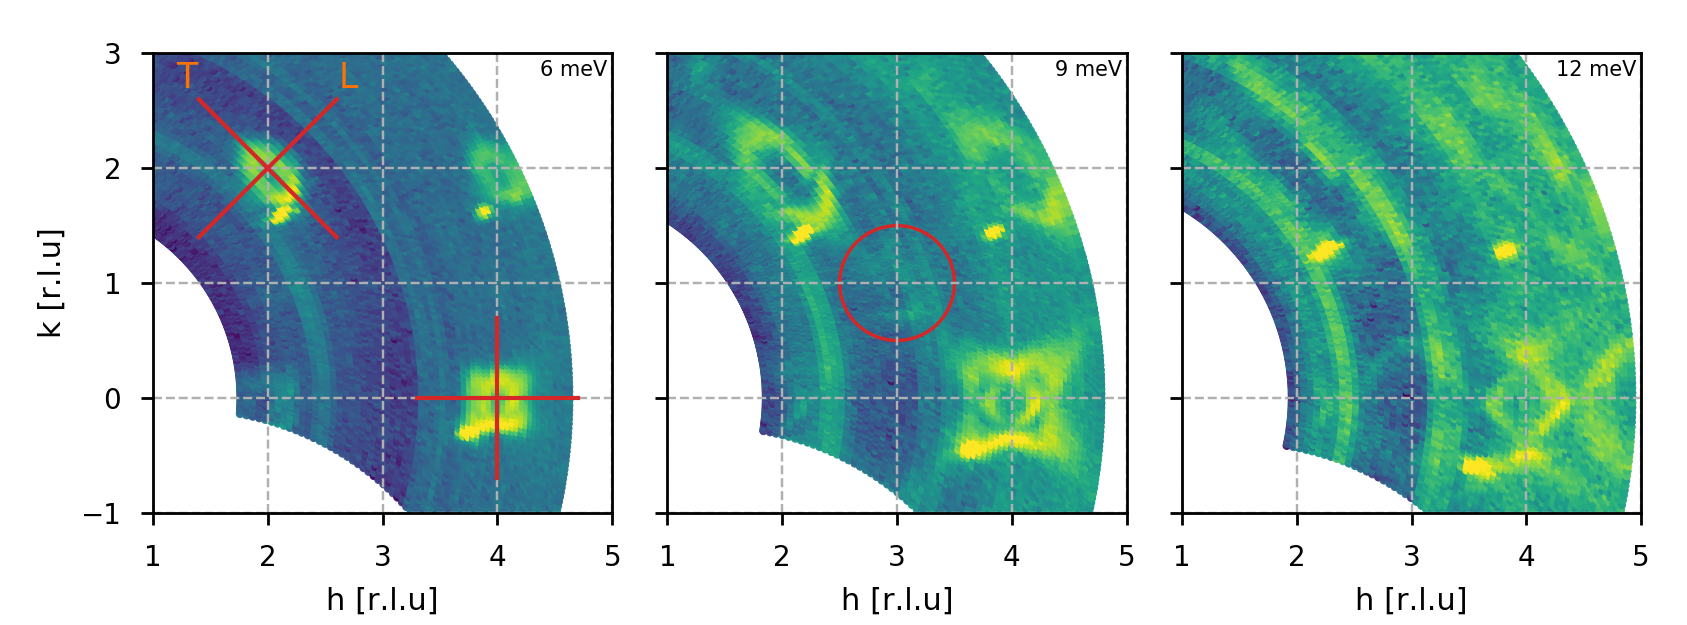
\includegraphics[width=\textwidth]{fig/lowen/flatcone_colorplots.png}
    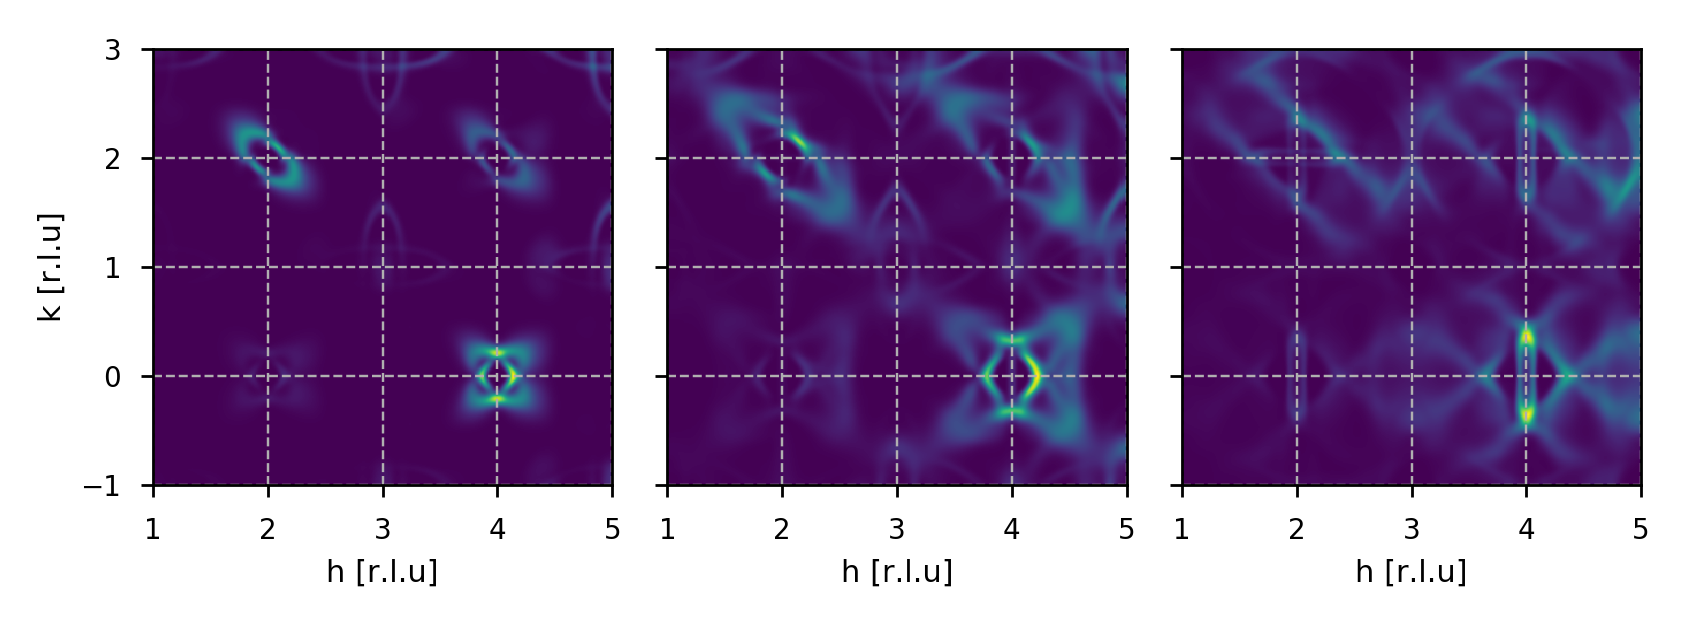
\includegraphics[width=\textwidth]{fig/lowen/simulation_colorplots.png}
    \caption[Flatcone raw inelastic]{Flatcone raw inelastic}
    \label{fig:flatcone_raw_inelastic}
\end{figure}

\begin{figure}
    \centering
    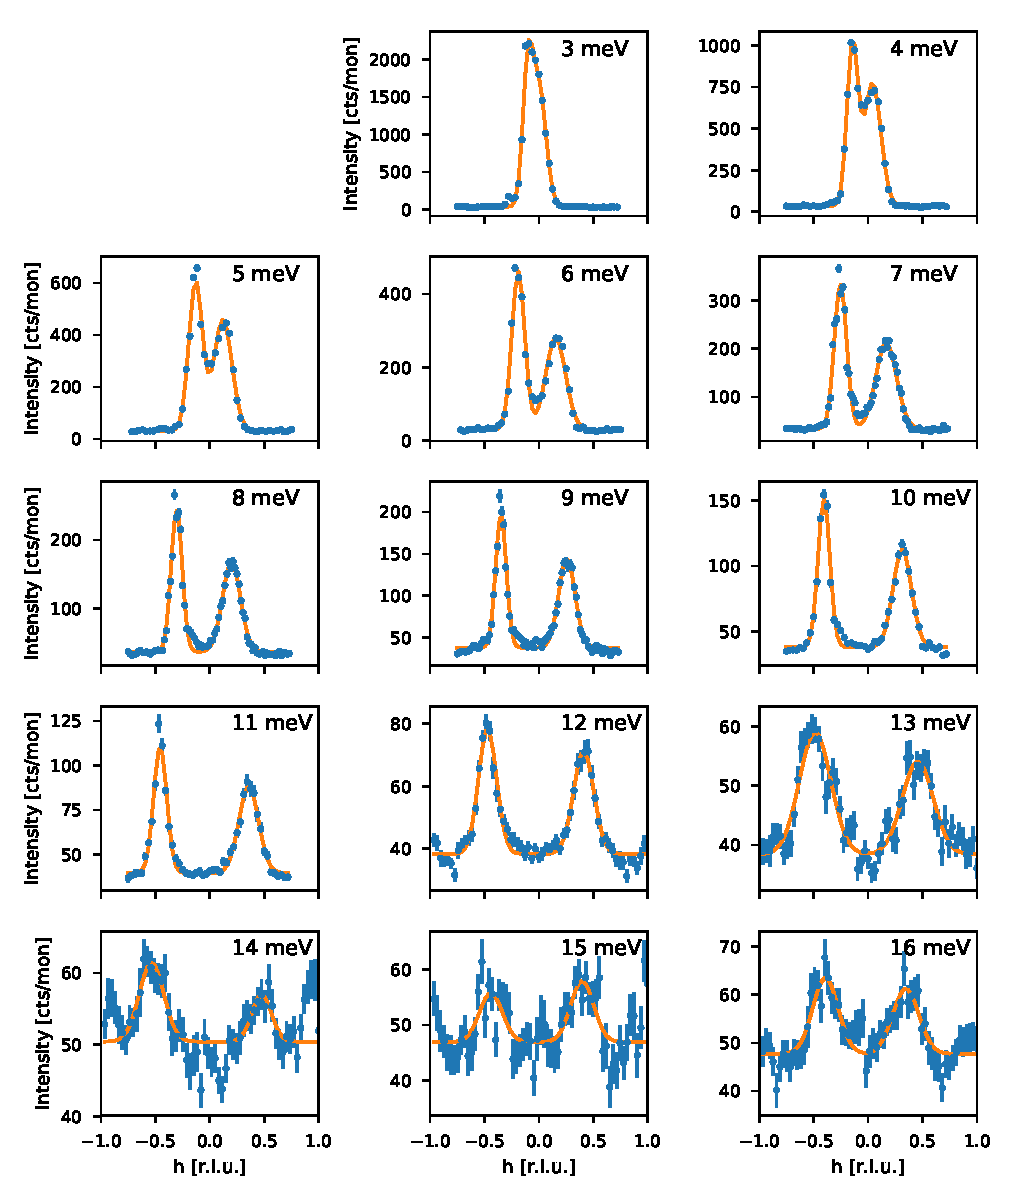
\includegraphics[width=\textwidth]{fig/lowen/fits_400T.pdf}
    \caption[400T flatcone raw data]{400T flatcone raw data}
    \label{fig:flatcone_phonons_400T_raw}    
\end{figure}

\begin{figure}
    \centering
    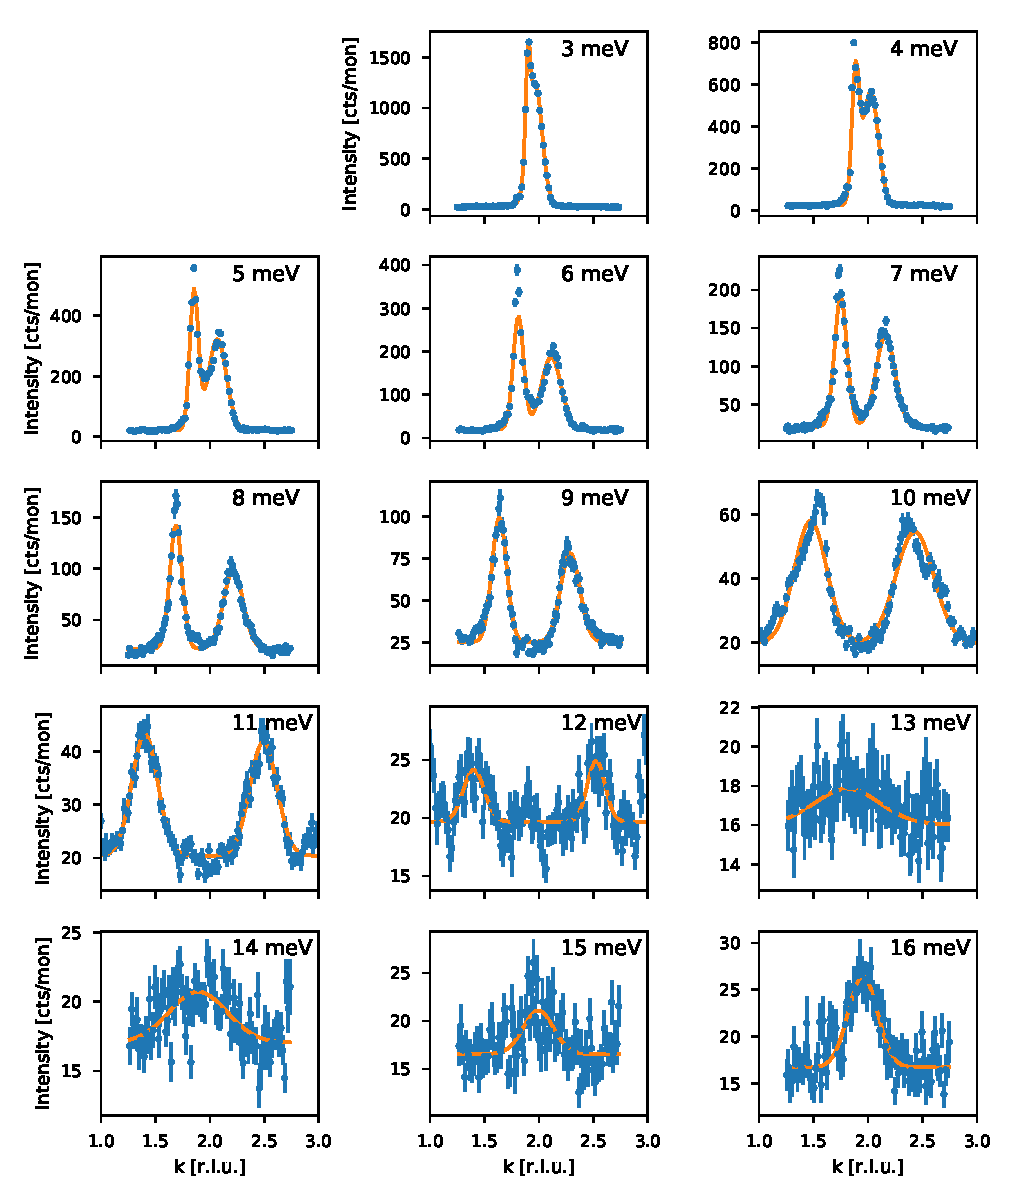
\includegraphics[width=\textwidth]{fig/lowen/fits_220T.pdf}
    \caption[220T flatcone raw data]{220T flatcone raw data}
    \label{fig:flatcone_phonons_400T_raw}    
\end{figure}

\begin{figure}
    \centering
    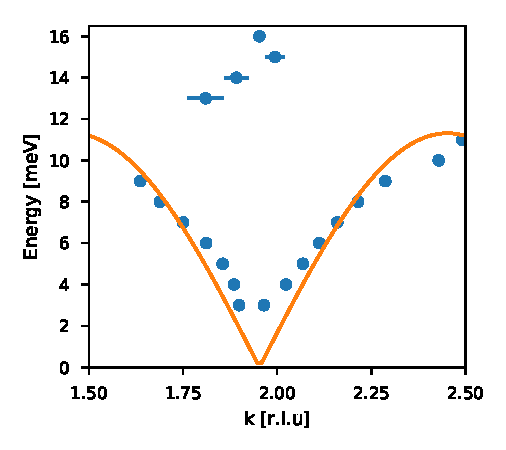
\includegraphics[width=0.45\textwidth]{fig/lowen/dispersion_220T.pdf}
    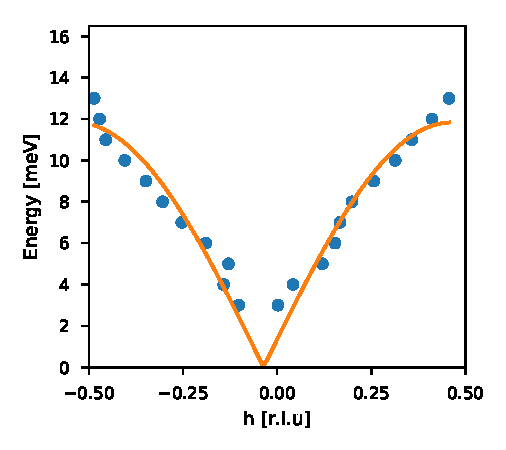
\includegraphics[width=0.45\textwidth]{fig/lowen/dispersion_400T.pdf}
    \caption[flatcone dispersion 220T/400T]{transverse flatcone dispersions at 220 (left) and 400 (right). Fit is a simple acoustic phonon dispersion for monoatomic systems: $\omega = \sqrt{4C/M} | \sin ( \pi (q-q_0) ) | $, where $M$ is the mass $C$ is the spring constant and $q_0$ is an offset to adjust for possible misalignment of the sample. $q$ is in reciprocal lattice units.}
\end{figure}

\begin{figure}
    \centering
    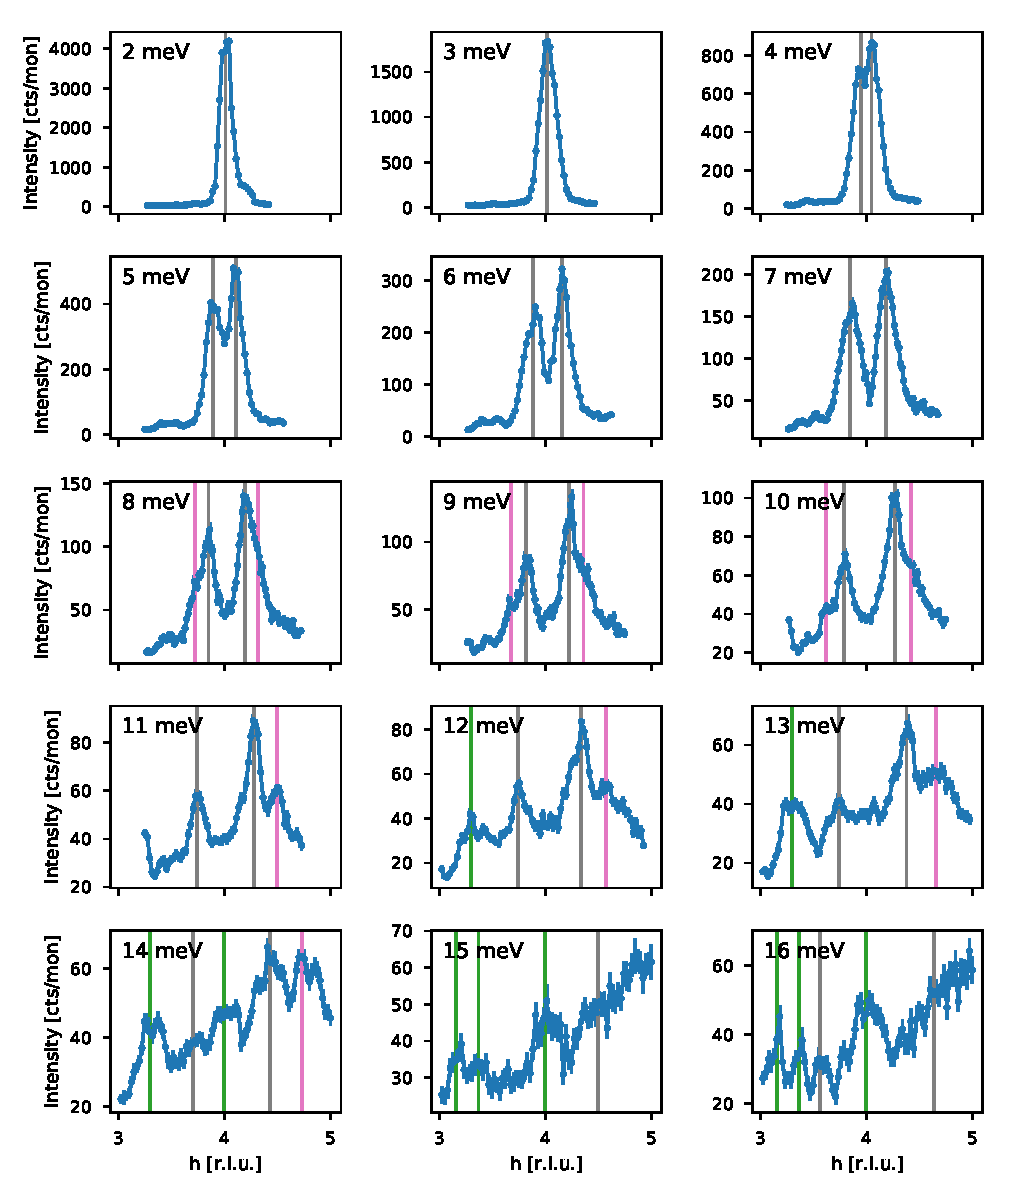
\includegraphics[width=\textwidth]{fig/lowen/fits_400L.pdf}
    \caption[400L flatcone raw data]{400L flatcone raw data}
    \label{fig:flatcone_phonons_400L_raw}    
\end{figure}

\begin{figure}
    \centering
    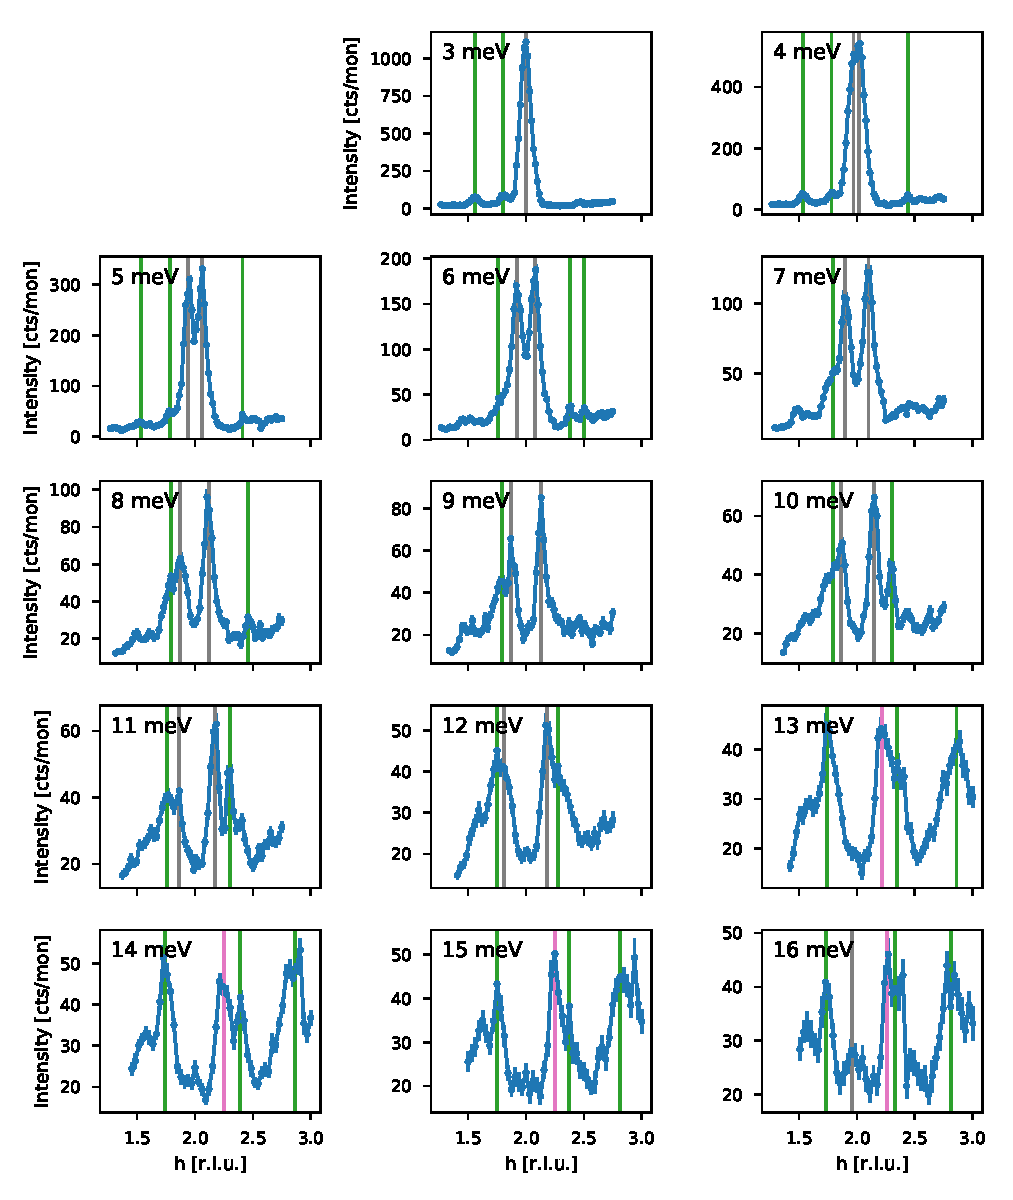
\includegraphics[width=\textwidth]{fig/lowen/fits_220L.pdf}
    \caption[220L flatcone raw data]{220L flatcone raw data}
    \label{fig:flatcone_phonons_220L_raw}    
\end{figure}

\begin{figure}
    \centering
    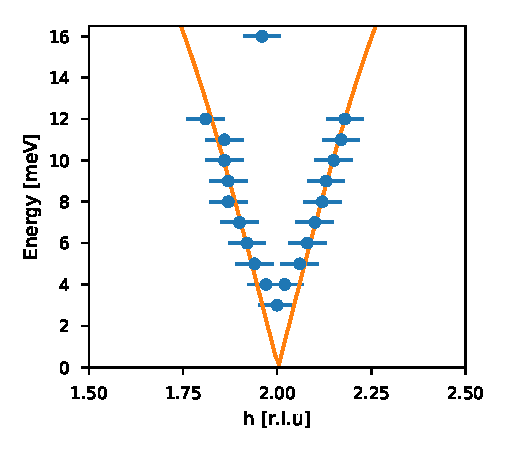
\includegraphics[width=0.45\textwidth]{fig/lowen/dispersion_220L.pdf}
    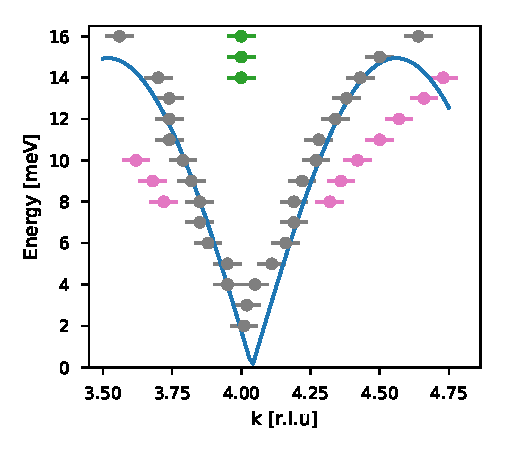
\includegraphics[width=0.45\textwidth]{fig/lowen/dispersion_400L.pdf}
    \caption[flatcone dispersion 220L/400L]{Longitudinal flatcone dispersions at 220 (left) and 400 (right). Fit is a simple acoustic phonon dispersion for monoatomic systems: $\omega = \sqrt{4C/M} | \sin ( \pi (q-q_0) ) | $, where $M$ is the mass $C$ is the spring constant and $q_0$ is an offset to adjust for possible misalignment of the sample. $q$ is in reciprocal lattice units.}
\end{figure}

\begin{figure}
    \centering
    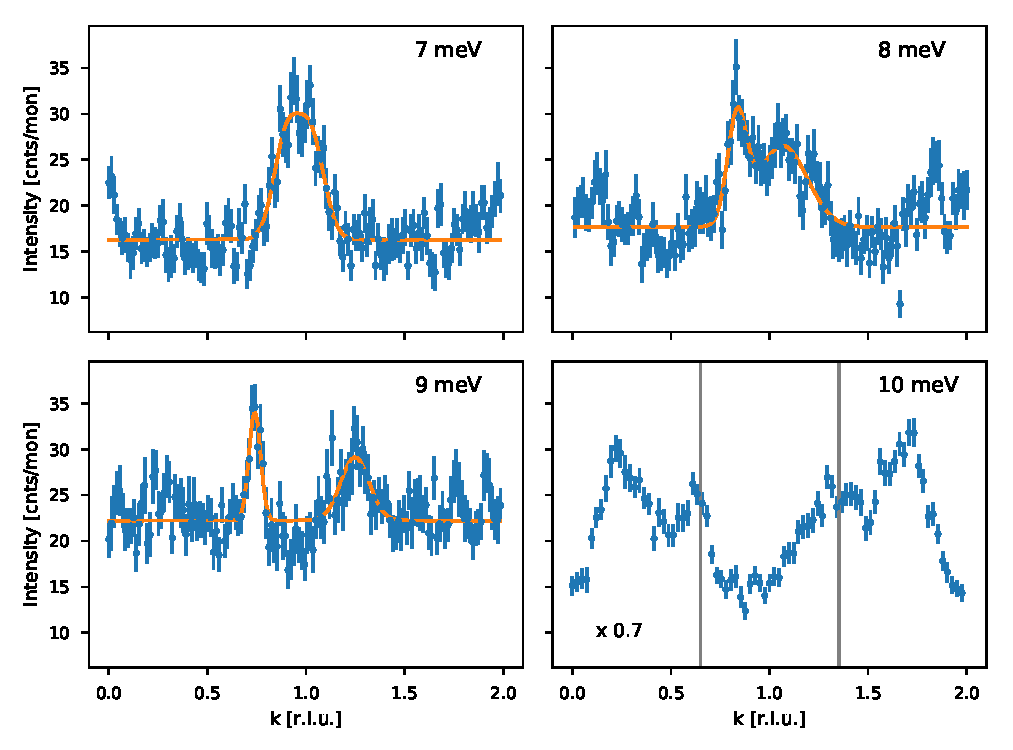
\includegraphics[width=\textwidth]{fig/lowen/fits_310T.pdf}
    \caption[310T flatcone raw data]{310T flatcone raw data. The dispersion appears quite flat: $\delta_k = \{ 0.06, 0.12, 0.25, 0.35 \}$ for the 4 energies shown, with the last one (\SI{10}{\milli\eV}) being a very rough estimate from visual inspection.}
    \label{fig:flatcone_phonons_310T_raw}    
\end{figure}

\begin{figure}[]
    \centering
    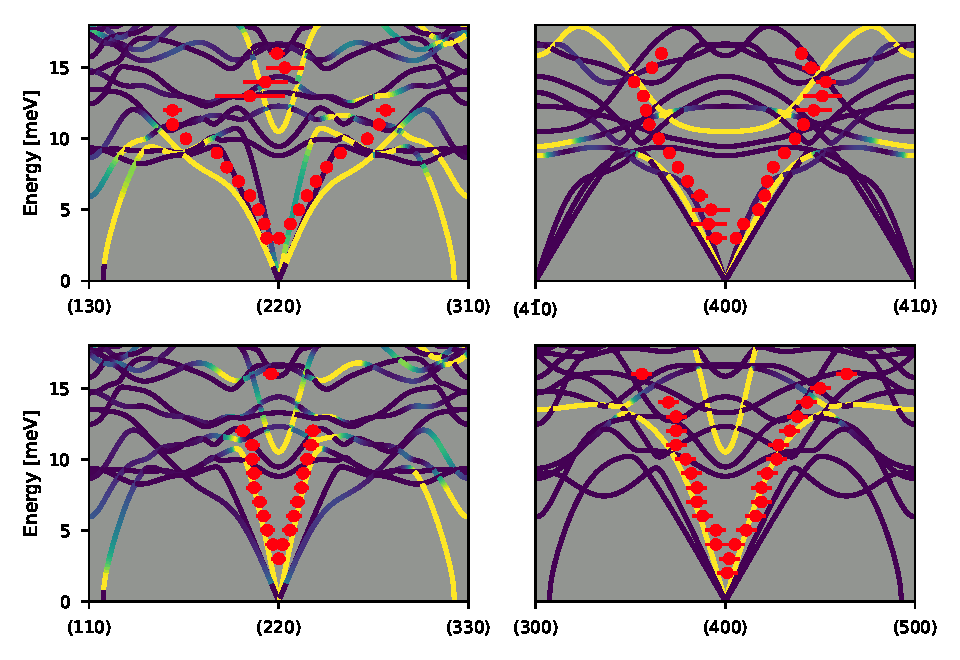
\includegraphics[width=\textwidth]{fig/lowen/flatcone_fits_simulation_afm.pdf}
    \caption[Flatcone dispersion and neutron weighted simulation data]{Flatcone dispersion and neutron weighted simulation data. LTO AFM simulation data.}
    \label{fig:flatcone_phonons_dispersion_simulation}
\end{figure}

\begin{figure}[]
    \centering
    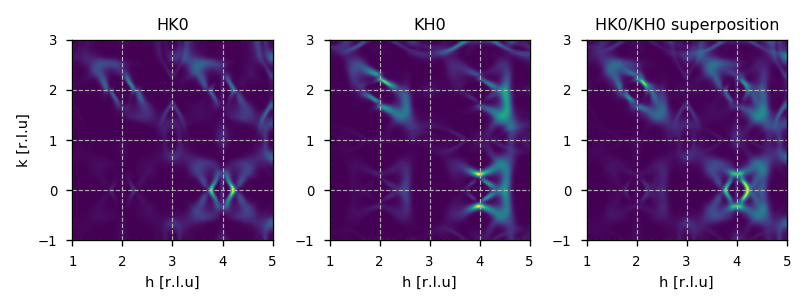
\includegraphics[width=\textwidth]{fig/lowen/simulation_colorplot_twin_comparison.png}
    \caption[Simulation comparison hkl khl]{Simulation comparison hkl khl and twin superposition}
    \label{fig:lto_hk0_kh0_comparison}
\end{figure}

\begin{figure}[]
    \centering
    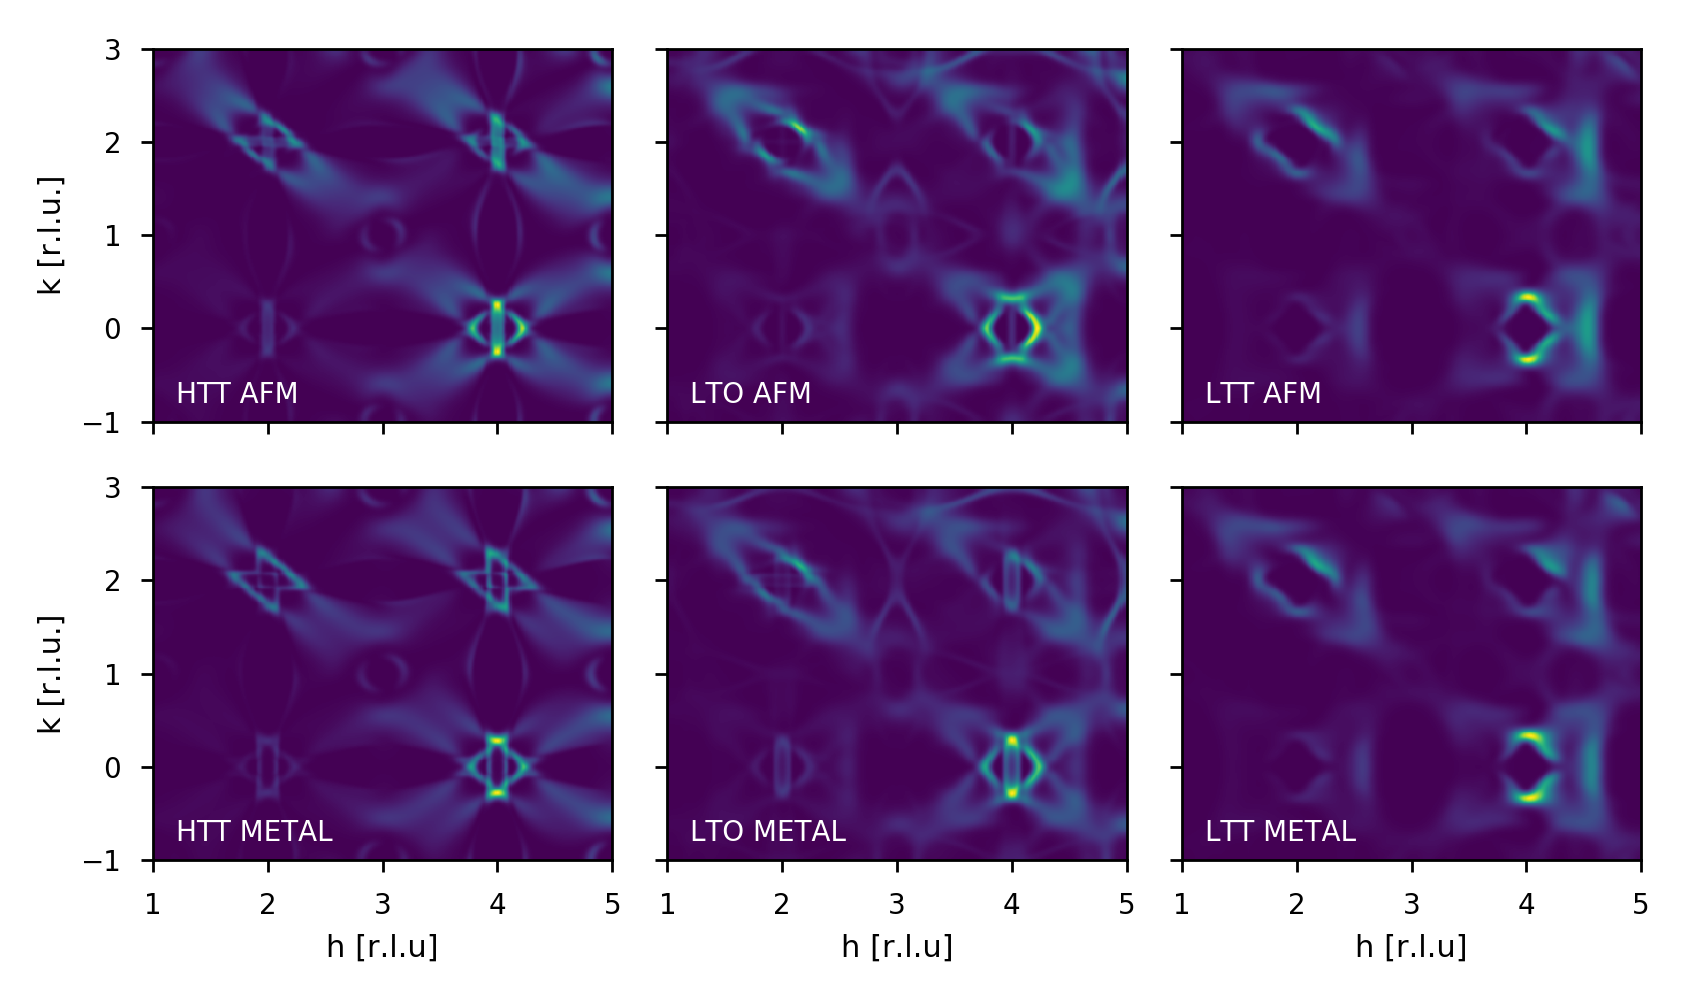
\includegraphics[width=\textwidth]{fig/lowen/twinning_plots_all.png}
    \caption[All qxqy plots at 9 meV including twinning for the LTO case]{All qxqy plots at 9 meV including twinning for the LTO case}
    \label{fig:simulation_sqw_xy_plots_all}
\end{figure}

\begin{figure}
    \centering
    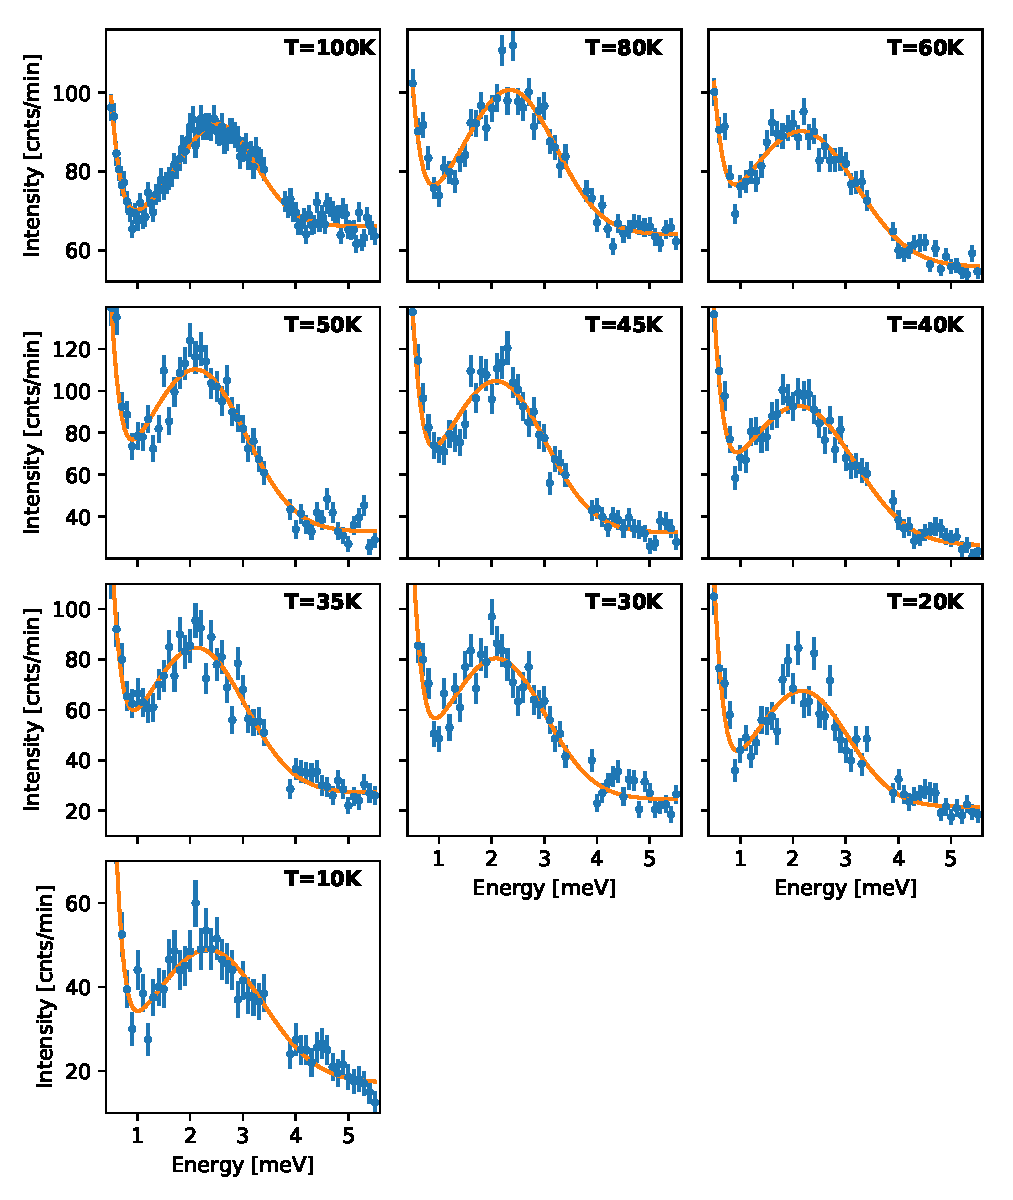
\includegraphics[width=\textwidth]{fig/lowen/lcoo_phonon_fits.pdf}
    \caption[lco+o Z-point phonon fits]{lco+o Z-point phonon fits}
    \label{fig:lcoo_zpoint_phonon_fits}
\end{figure}

\begin{figure}
    \centering
    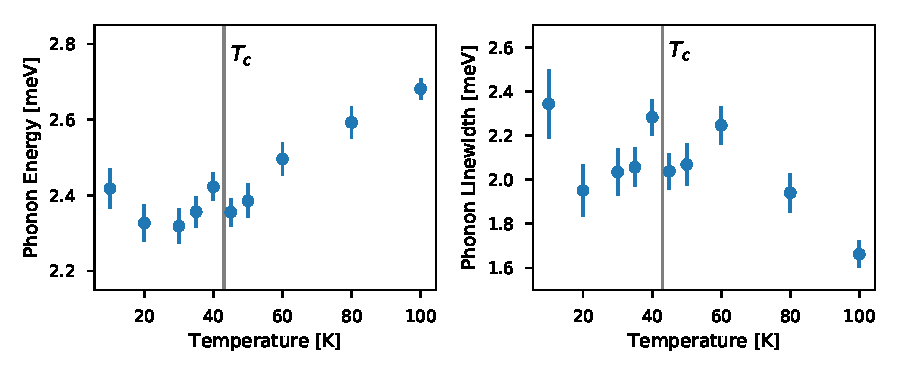
\includegraphics[width=\textwidth]{fig/lowen/lcoo_phonon_energies.pdf}
    \caption[lco+o Z-point phonon E-T plot]{lco+o Z-point phonon E-T plot}
    \label{fig:lcoo_zpoint_phonon_energies}
\end{figure}

\begin{figure}
    \centering
    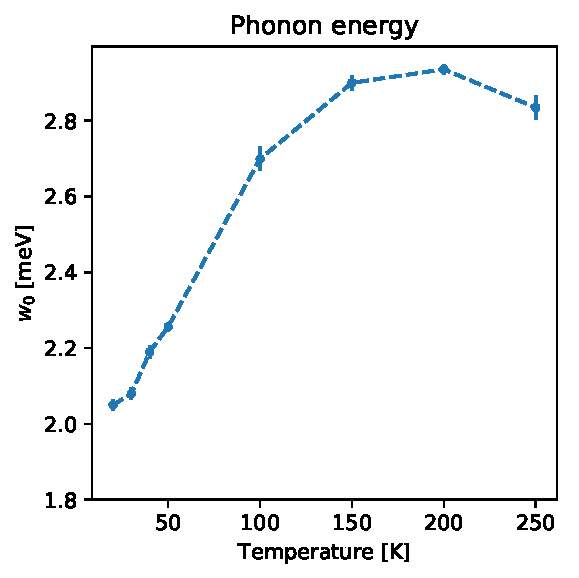
\includegraphics[width=0.45\textwidth]{fig/lowen/lsco5_phonon_energy.pdf}
    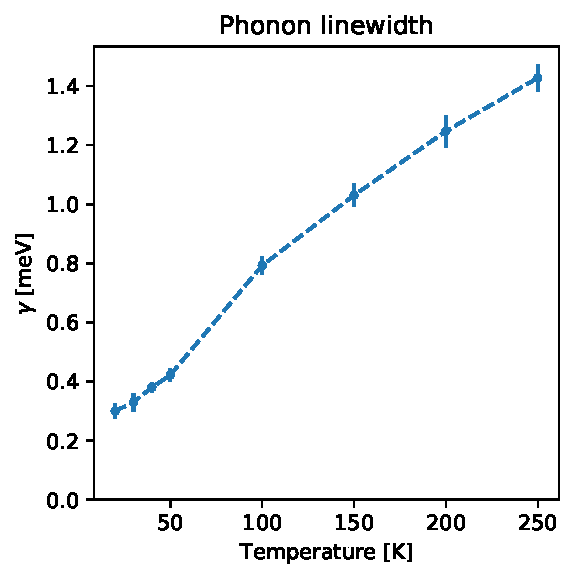
\includegraphics[width=0.45\textwidth]{fig/lowen/lsco5_phonon_linewidth.pdf}
    \caption[lsco5 z-point phonon E-T plot]{lsco5 z-point phonon E-T plot}
    \label{fig:lsco5_zpoint_phonon_energies}
\end{figure}

\begin{figure}
    \centering
    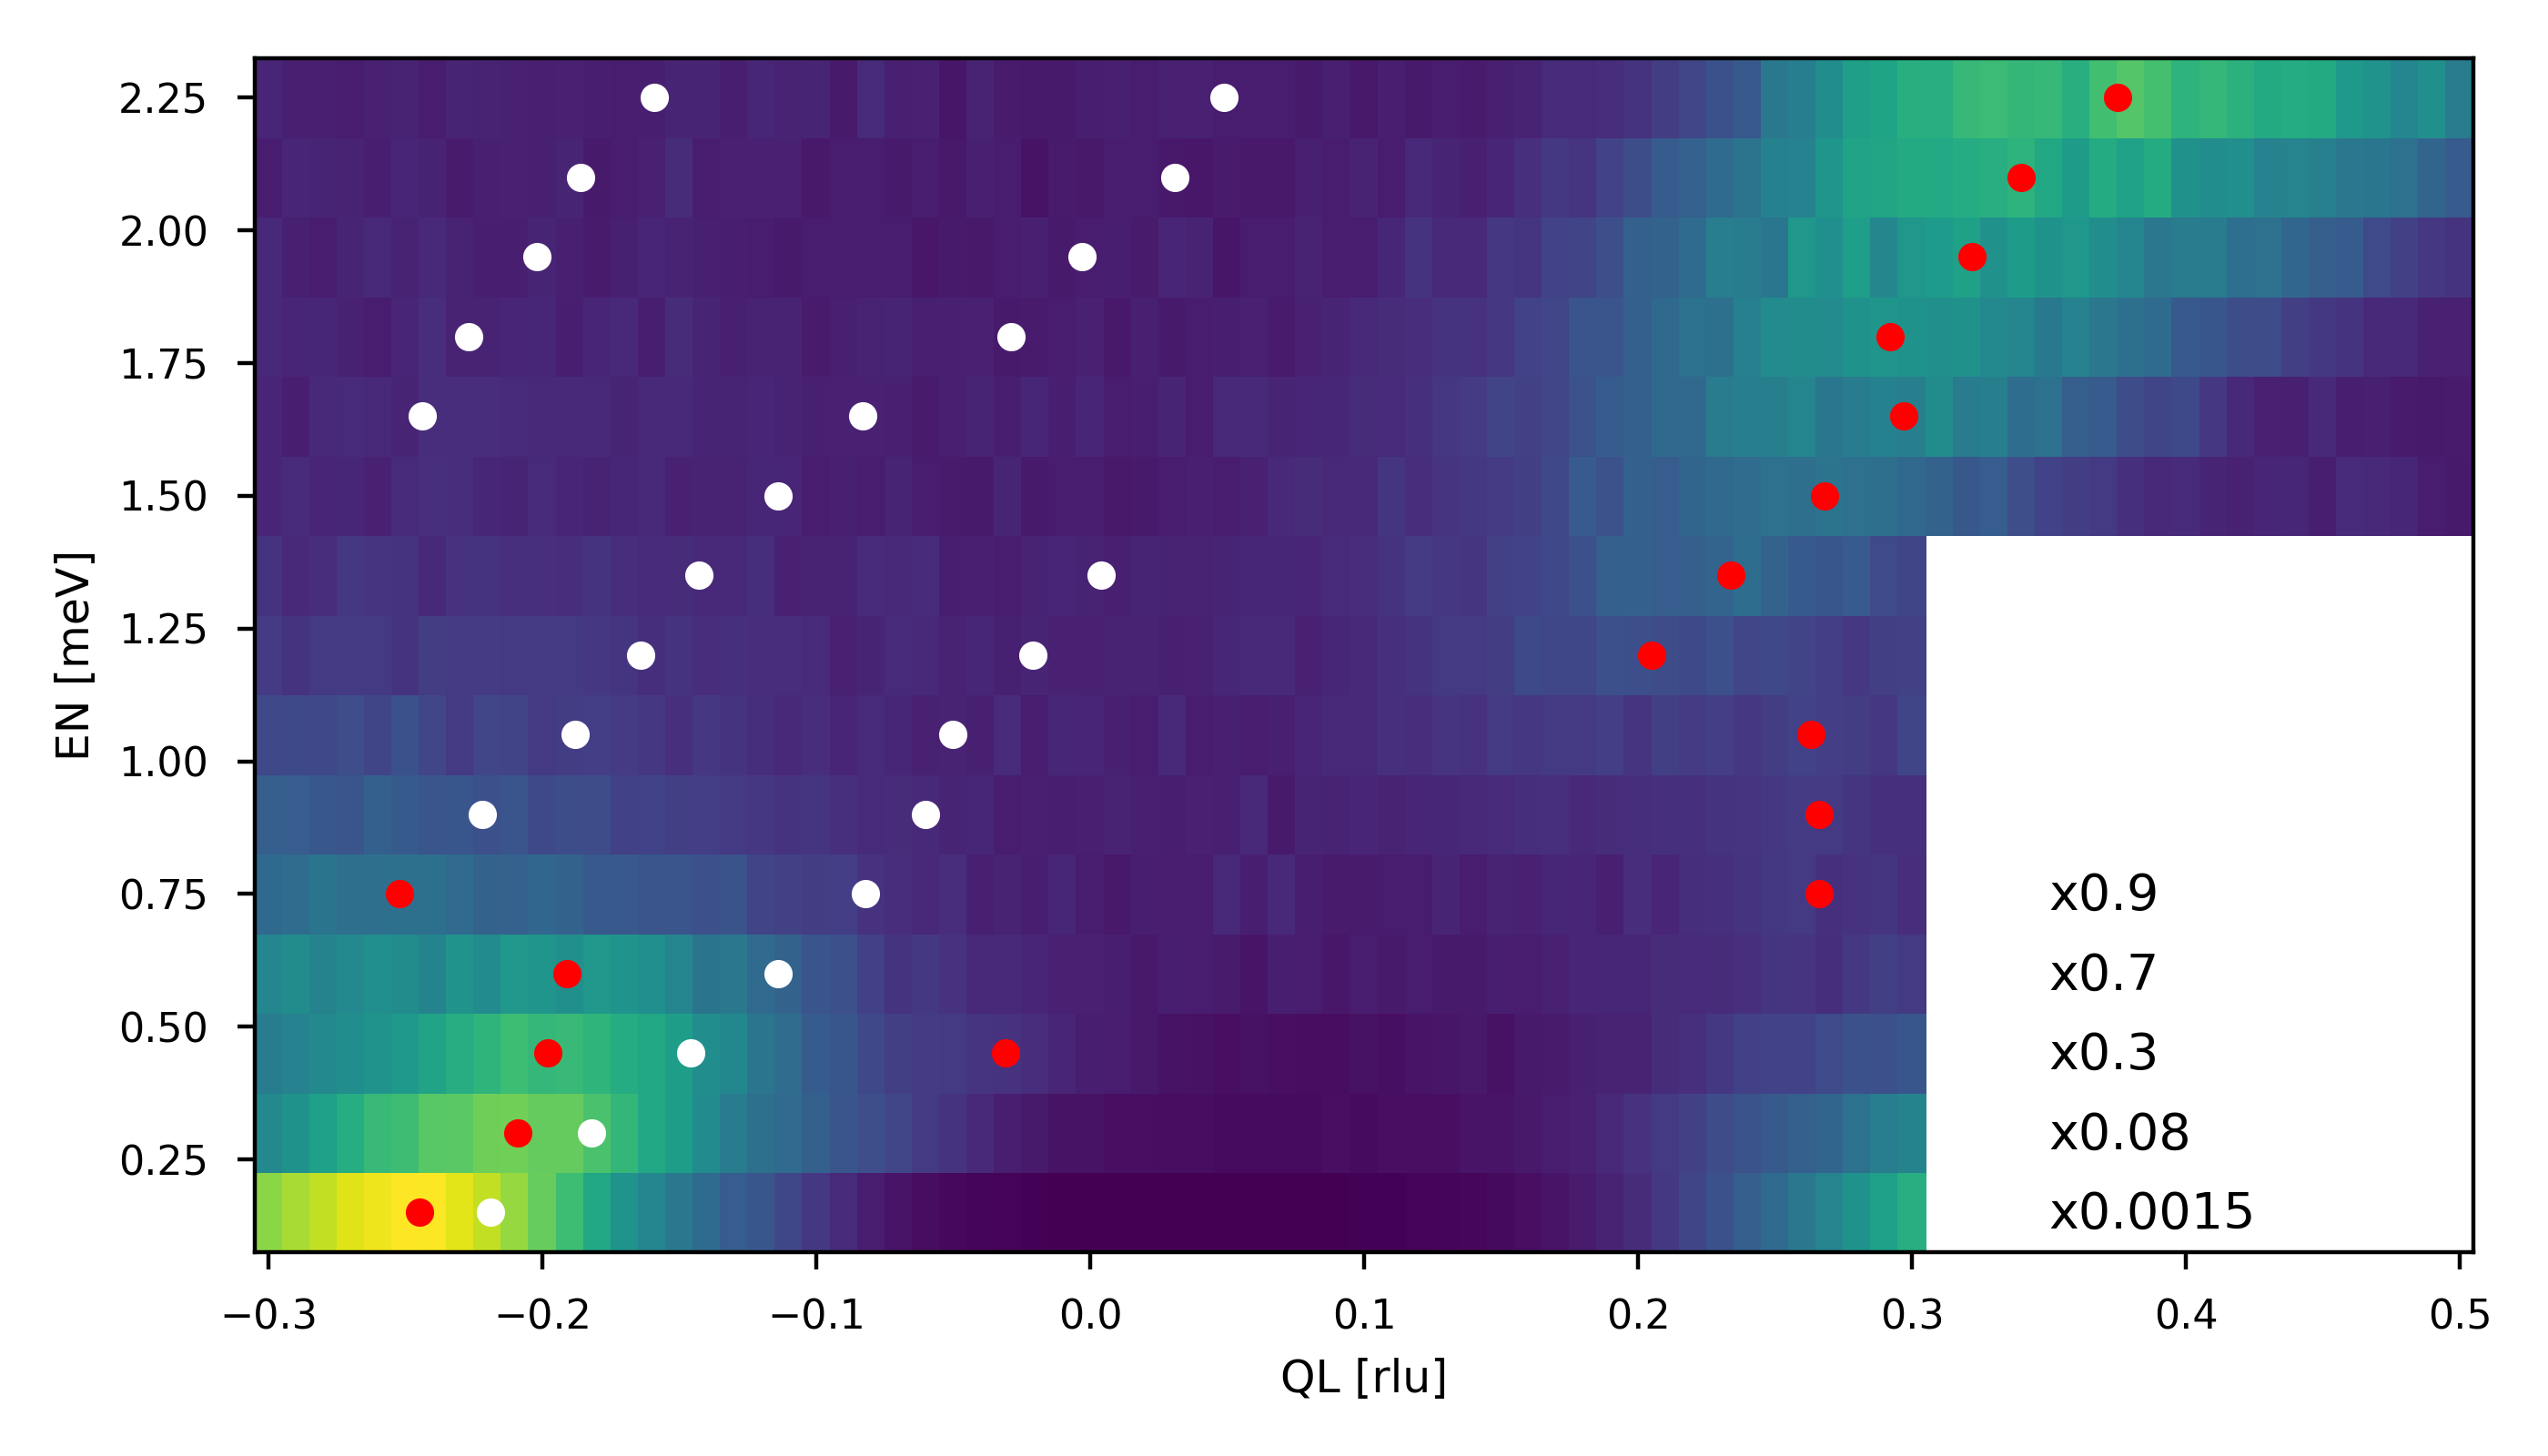
\includegraphics[width=0.85\textwidth]{fig/lowen/phason_colorplot.png}
    \caption[lack of phasons]{lack of phasons}
    \label{fig:lcoo_phasons_colorplot}
\end{figure}
